\documentclass[12pt]{article}
\usepackage{import}
\usepackage[margin=0.5in]{geometry}
\usepackage{graphics}
\usepackage{xcolor}


\graphicspath{{images/}}

\import{./}{python_highlights.tex}
\import{./}{polish.tex}
\import{./}{math_preambule.tex}

% Gray text box with shadow
\usepackage[skins]{tcolorbox}
\newenvironment{shbox}
{\begin{tcolorbox}[enhanced, boxrule=0pt, drop fuzzy shadow southeast]}
{\end{tcolorbox}}

\title{
    \huge Podstawy Sterowania Optymalnego - Labolatorium 1\\
    \large Wprowadzenie do języka Python
}
\author{Prowadzący: mgr inż. Krzysztof Hałas\\
        Wykonał: Ryszard Napierała}
\date{23 Październik 2021}
\setlength{\parindent}{15pt}

\begin{document}
    \maketitle

    \section{Zadanie 2}
    \begin{enumerate}
        \item\textbf{Wykorzystując Pythona oraz środowisko Spyder wyznaczyć wartość x.}
            \begin{enumerate}
                \item $x=3^{12}-5$\\
                \python{snippets/lab1/zad2_1_1.py}
                \begin{shbox}
                    \textbf{Output:} 531436
                \end{shbox}
                \item $x=
                    \begin{bmatrix}
                        2& 5
                    \end{bmatrix}
                    \begin{bmatrix}
                        1& 4\\
                        -1& 3
                    \end{bmatrix}
                    \begin{bmatrix}
                        -1\\
                        -3
                    \end{bmatrix}$\\
                    \python{snippets/lab1/zad2_1_2.py}
                    \begin{shbox}
                        \textbf{Output:} $[[-30.]]$
                    \end{shbox}
                \item $x=rank(
                    \begin{bmatrix}
                        1& -2& 0\\
                        -2& 4& 0\\
                        2& -1& 7
                    \end{bmatrix})$\\
                    \python{snippets/lab1/zad2_1_3.py}
                    \begin{shbox}
                        \textbf{Output:} $2$
                    \end{shbox}
                \item $
                    \begin{bmatrix}
                        -1\\
                        2
                    \end{bmatrix} =
                    \begin{bmatrix}
                        1& 2\\
                        -1& 0
                    \end{bmatrix} x$\\
                    \python{snippets/lab1/zad2_1_4.py}
                    \begin{shbox}
                        \textbf{Output:} \\
                        $[[-2. ]$\\
                        $[ 0.5]]$
                    \end{shbox}
            \end{enumerate}
            \item\textbf{Dana jest tablica [1, 1, -129, 1620]. Napisać skrypt tworzący zmienną przechowującą
            tę tablicę. Przyjmując zawartość tablicy jako współczynniki wielomianu (zaczynając od
            najwyższej potęgi) wyznaczyć wartość tego wielomianu w punktach $x_1=-46, x_2=14$.}
            \python{snippets/lab1/zad2_2.py}
            \begin{shbox}
                \textbf{Output:} \\
                dla $x=-46$, $y=4100910$\\
                dla $x=14$, $y=19890$
            \end{shbox}
        \end{enumerate}

    \section{Zadanie 3}
        \begin{enumerate}
            \item\textbf{Bazując na poprzednim zadaniu rozbudować skrypt tak, by w sposób numeryczny wyznaczył
            największą i najmniejszą wartość wielomianu w przedziale} $
                \begin{bmatrix}
                    -46&14
                \end{bmatrix}$.
                \python{snippets/lab1/zad3_1.py}
                \begin{shbox}
                    \textbf{Output:} \\
                    $[ -4536.\text{ } 4100910.]$
                \end{shbox}

            \item\textbf{Uzależnić dokładność wyznaczania ekstremów od wartości dodatkowej zmiennej.}
                \python{snippets/lab1/zad3_2.py}
                \begin{shbox}
                    \textbf{Output:} \\
                    $[ -4561.29354219\text{ } 4100910.]$
                \end{shbox}
        \end{enumerate}
        
    \section{Zadanie 4}
    \begin{enumerate}
            \item\textbf{Zmodyfikować skrypt z poprzedniego zadania tak,
                by funkcjonalność wyznaczająca maksimmum i minimum wielomianu
                zawarta była w funkcji przyjmującej współczynniki wielomianu 4 stopnia,
                granice wyznaczania oraz wskaźnik dokładności jako argumenty.
                Wyznaczone wartości minimum i maksimum powinny być zwracane jako tablica dwuelementowa.}
                \python{snippets/lab1/zad4_1.py}
                \begin{shbox}
                    \textbf{Output:} \\
                    $[ -4561.29354219\text{ } 4100910.]$
                \end{shbox}

            \item\textbf{Rozbudować skrypt, by funkcja przyjmowała jako argument
                tablicę współczynników wielomianu dowolnego stopnia.}
                \python{snippets/lab1/zad4_2.py}
                \begin{shbox}
                    \textbf{Output:} \\
                    $[ -4561.29354219\text{ } 4100910.]$
                \end{shbox}
        \end{enumerate}
        
    \section{Zadanie 5}
        \begin{enumerate}
            \item\textbf{Zmodyfikować skrypt z poprzedniego zadania tak,
                funkcja wyznaczająca ekstrema wielomianu wykreślała
                przebieg wielomianu w całym wymaganym zakresie. }
                \python{snippets/lab1/zad5_1.py}
                \begin{shbox}
                    \centering
                    \textbf{Output:} \\
                    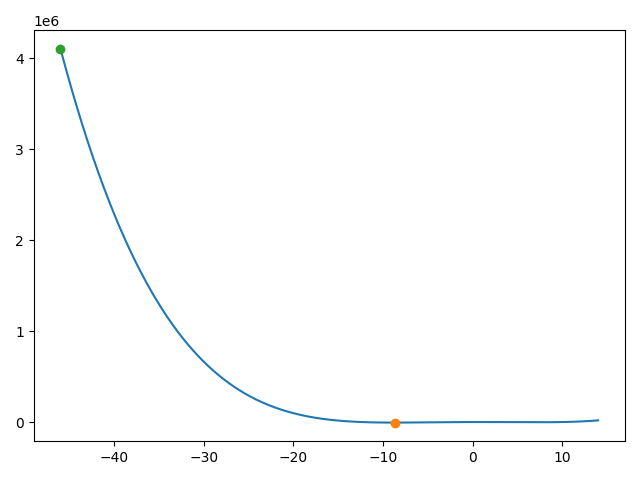
\includegraphics[width=0.75\textwidth]{zad5_1.png}
                \end{shbox}

            \item\textbf{Dodać do generowanego wykresu legendę, opisy osi, tytuł, itp.}
                \python{snippets/lab1/zad5_2.py}
                \begin{shbox}
                    \centering
                    \textbf{Output:} \\
                    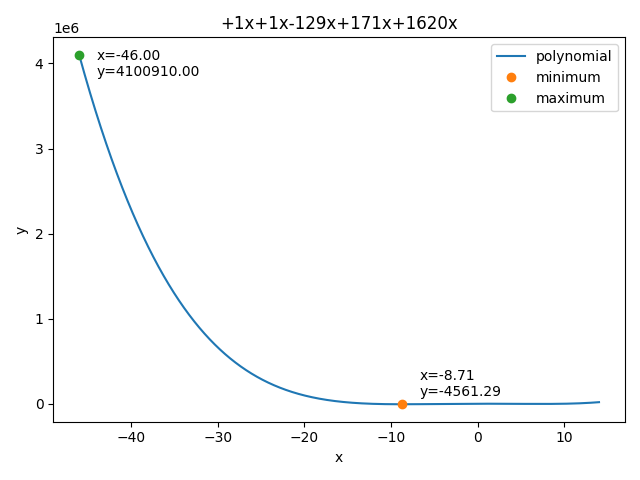
\includegraphics[width=0.75\textwidth]{zad5_2.png}
                \end{shbox}
        \end{enumerate}

\end{document}